% !TEX program = xelatex
% !TeX spellcheck = ru_RU_yo

\documentclass[xetex,с,aspectratio=169]{beamer}

\usepackage{xecyr}
\usepackage{xunicode}
\usepackage{fontspec}
\defaultfontfeatures{Ligatures=TeX}
\setmainfont{ALSSchlangesans}

\usepackage{polyglossia}
\setdefaultlanguage[spelling=modern]{russian}
\newfontfamily{\cyrillicfont}[BoldFont={*-Bold}]{ALSSchlangesans}
\newfontfamily{\cyrillicfontsf}[BoldFont={*-Bold}]{ALSSchlangesans}
\newfontfamily{\cyrillicfonttt}{Droid Sans Mono}

\usepackage[euler-digits,small]{eulervm}
\AtBeginDocument{\renewcommand{\hbar}{\hslash}}

\definecolor{ifmoblue}{RGB}{25,70,186}
\definecolor{ifmored}{RGB}{236,11,67}

\setbeamertemplate{itemize items}[circle]

\usepackage{epstopdf}
\usepackage{graphicx}
\usepackage{amsmath}
\usepackage{nicefrac}
\usepackage{ctable}
\usepackage{ragged2e}

\usepackage{pifont}
\newcommand{\cmark}{\ding{51}}%
\newcommand{\xmark}{\ding{55}}%


\usepackage{xcolor}
\newcommand{\highlight}[1]{\colorbox{orange!50}{$\displaystyle#1$}}

\usepackage{textpos}

\newcommand{\email}[1]{{\scriptsize\texttt{#1}}}

\usebackgroundtemplate{}

\titlegraphic{
\includegraphics[width=5cm]{ifmo/logo-blue}}
\title{Разработка веб-приложения для работы с программным пакетом высокоточного позиционирования RTKLIB}
\author[Кузнецов А.А., P3410]{Кузнецов Андрей Андреевич, ПИиКТ, ИПМ, Р4215}
\date[]{Научный руководитель: Соснин В.В., к.т.н., доцент}

\usetheme{ifmo}
\setbeamersize{text margin left=0.6cm,text margin right=0.5cm}

\begin{document}

%
% Title
%
{
  \setbeamertemplate{footline}{}

  \begin{frame}
    \titlepage
  \end{frame}
}


%
% DGPS
%
\begin{frame}
  \frametitle{Дифференциальная GPS}
  
  \large

  \begin{center}
    \textbf{Дифференциальная GPS} -- система, предназначенная для повышения\\точности сигналов GPS.
  \end{center}

  \vskip -0.25cm

  \begin{figure}[h]
    \centering
    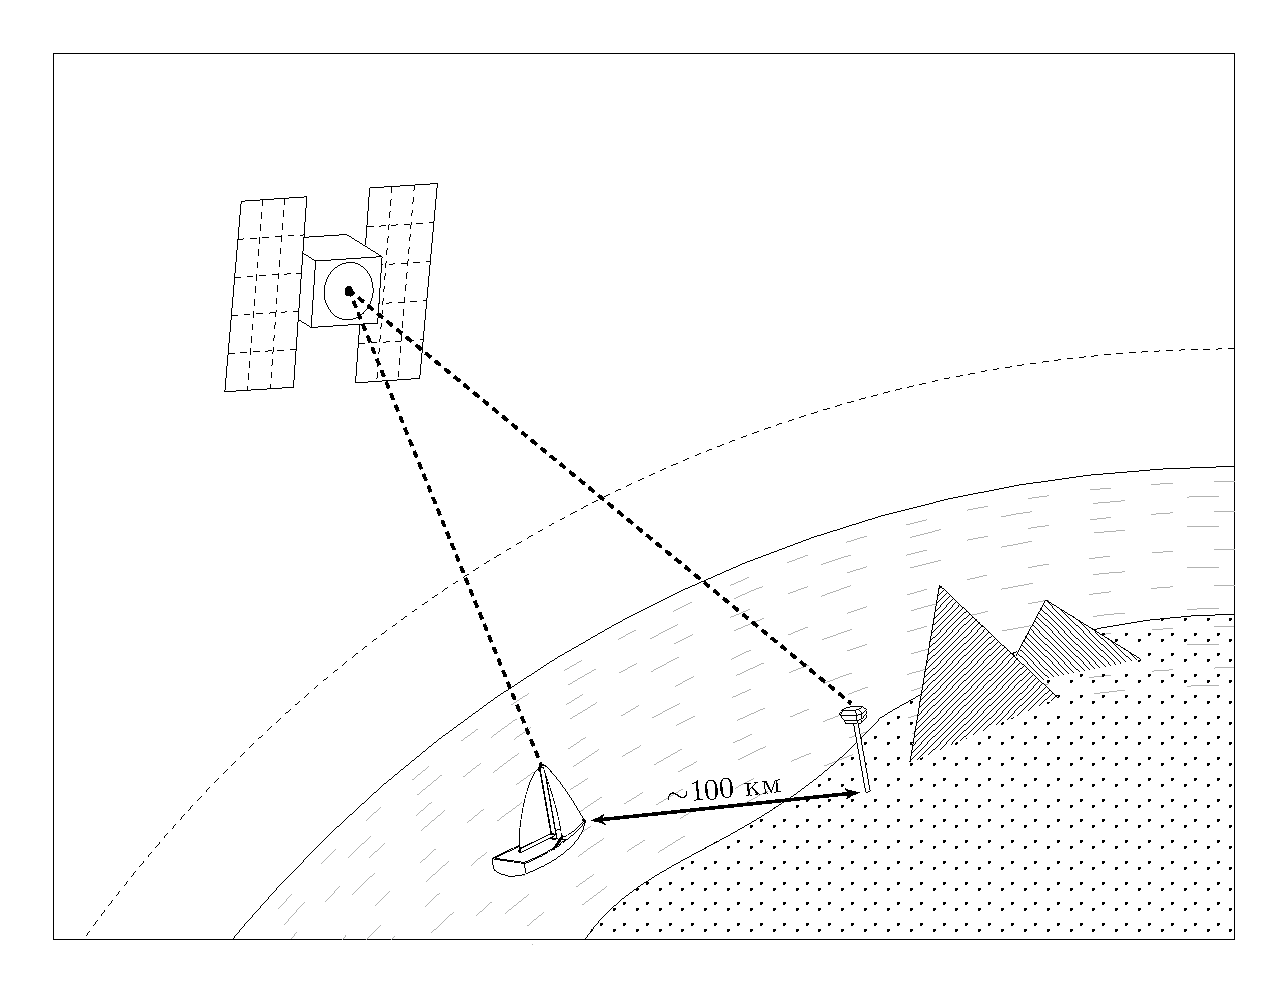
\includegraphics[height=5.5cm]{../img/tikz/dgps-one/pic}
  \end{figure}
\end{frame}


%
% RTK
%
\begin{frame}
  \frametitle{Кинематика реального времени}

  \Large

  \begin{center}
    \textbf{Кинематика реального времени} (англ. \emph{Real Time Kinematic, RTK}) -- режим работы, при котором приём и~применение поправок с~базы происходят в~реальном времени.
  \end{center}
  \vskip0.2cm
  \begin{center}
    \vskip -1cm
    \color{ifmoblue}{\rule{.5\textwidth}{0.5pt}}
  \end{center}

  \begin{minipage}{\textwidth}
    \centering
    \begin{minipage}[t]{.3\textwidth}
      \centering
      \begin{figure}[h]
        \centering
        
\includegraphics[height=21pt]{../img/trimble}
      \end{figure}
      \$~10$\,$000

      {
        \scriptsize
        \color{gray}{Trimble R8 Model 3 (2009)}
      }
    \end{minipage}
    \hspace{1em}
    \begin{minipage}[t]{.3\textwidth}
      \centering
      \begin{figure}[h]
        \centering
        
\includegraphics[height=21pt]{../img/leica}
      \end{figure}
      \$~6$\,$000

      {
        \scriptsize
        \color{gray}{Leica Viva GS08 (2012)}
      }
    \end{minipage}
  \end{minipage}
\end{frame}


%
% RTKLIB
%
\begin{frame}
  \frametitle{RTKLIB (\,1\,)}

  \Large

  \begin{center}
    \textbf{RTKLIB} -- программный пакет с~открытым исходным кодом, предназначенный для осуществления стандартного и~высокоточного позиционирования с~помощью глобальных навигационных спутниковых систем.
  \end{center}
  
  \begin{figure}[h]
    \centering
    
\includegraphics[height=2cm]{../img/rtklib}
  \end{figure}
\end{frame}


%
% RTKLIB problems
%
\begin{frame}
  \frametitle{RTKLIB (\,2\,)}
  \framesubtitle{Проблемы использования}

  \begin{figure}[h]
    \centering
    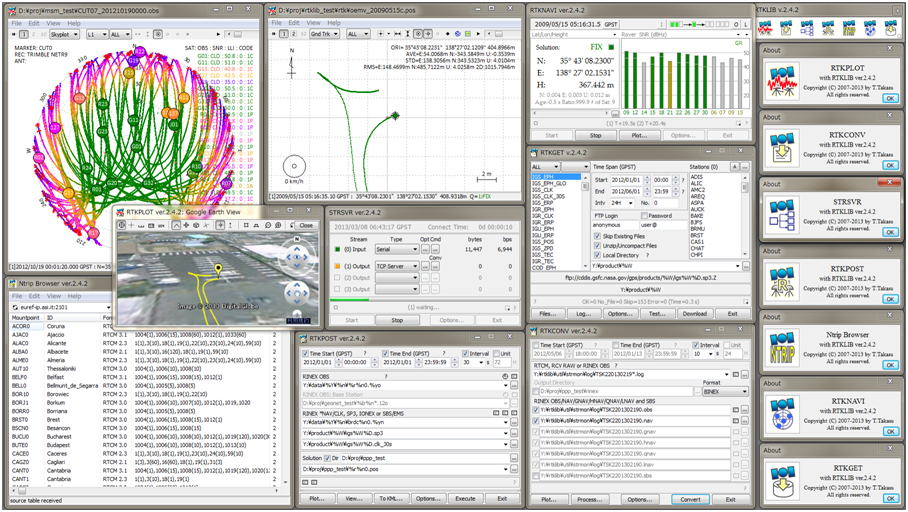
\includegraphics[width=.75\textwidth]{../img/rtklib-hell}
  \end{figure}
\end{frame}


%
% Main task
%
\begin{frame}
  \frametitle{Характеристика проведённой работы}
  \vskip 0.5cm
  \begin{center}
    {
      \Large
      \textbf{Объект исследования} -- программный пакет высокоточного позиционирования RTKLIB.
      \vskip .75cm
      \textbf{Предмет исследования} -- процесс взаимодействия пользователя с~программными компонентами RTKLIB.
      \vskip .75cm
      \textbf{Цель работы} -- создание веб-приложения для обеспечения\\взаимодействия пользователя с~программным пакетом RTKLIB,\\используемом во~встраиваемом решении.\\
    }
  \end{center}
\end{frame}


%
% Receivers review
%
{
  \usebackgroundtemplate{
    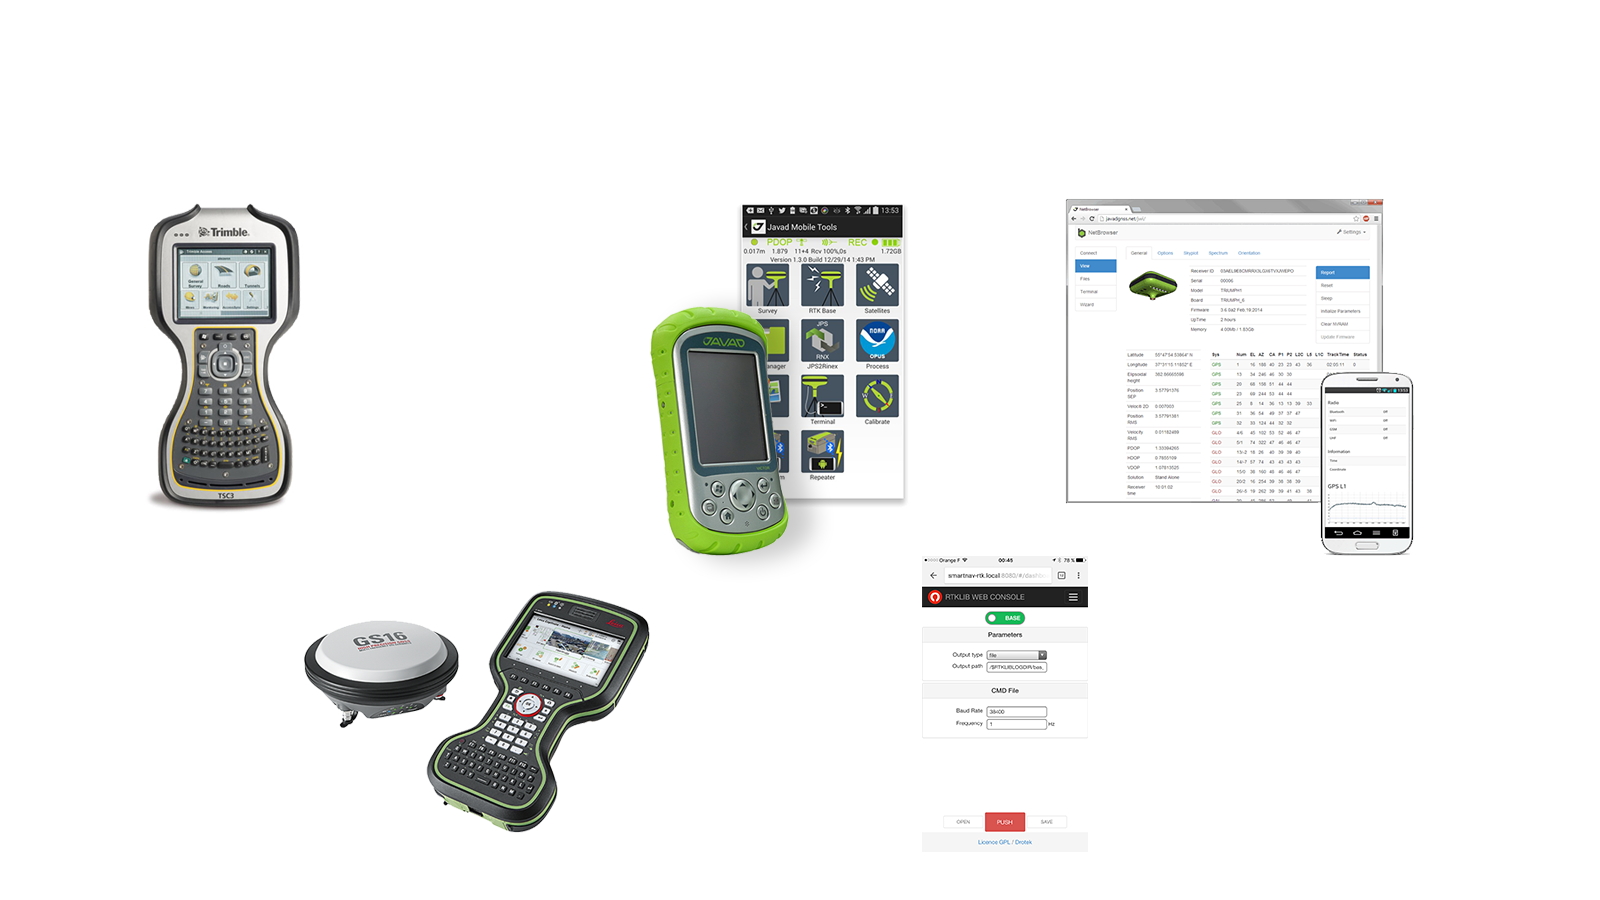
\includegraphics[width=\paperwidth]{../img/presentation/controllers}
  }

  \begin{frame}
    \frametitle{Обзор существующих решений (\,1\,)}
    \framesubtitle{Интерфейсы для управления приёмниками}
  \end{frame}
}

%
% Web apps review
%
\begin{frame}
  \frametitle{Обзор существующих решений (\,2\,)}
  \framesubtitle{Веб-интерфейсы для управления устройствами}
  \vskip 1cm
  \begin{minipage}{\textwidth}
    \centering
    \begin{minipage}[c]{.45\textwidth}
      \centering
      \begin{figure}[h]
        \centering
        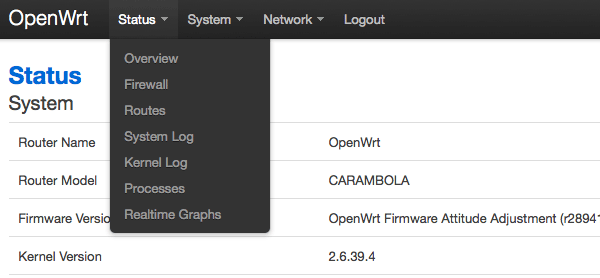
\includegraphics[width=\textwidth]{../img/openwrt-menu}
      \end{figure}
      OpenWrt
    \end{minipage}
    \hspace{1em}
    \begin{minipage}[c]{.45\textwidth}
      \centering
      \begin{figure}[h]
        \centering
        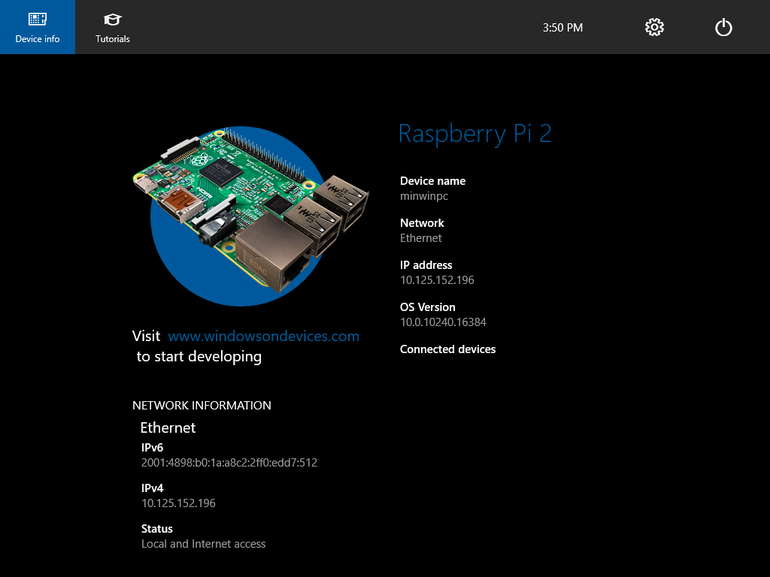
\includegraphics[width=\textwidth]{../img/win10-device-info}
      \end{figure}
      Windows 10 IoT Core
    \end{minipage}
  \end{minipage}
\end{frame}

%
% Reach & Reach RS
%
{
  \usebackgroundtemplate{
    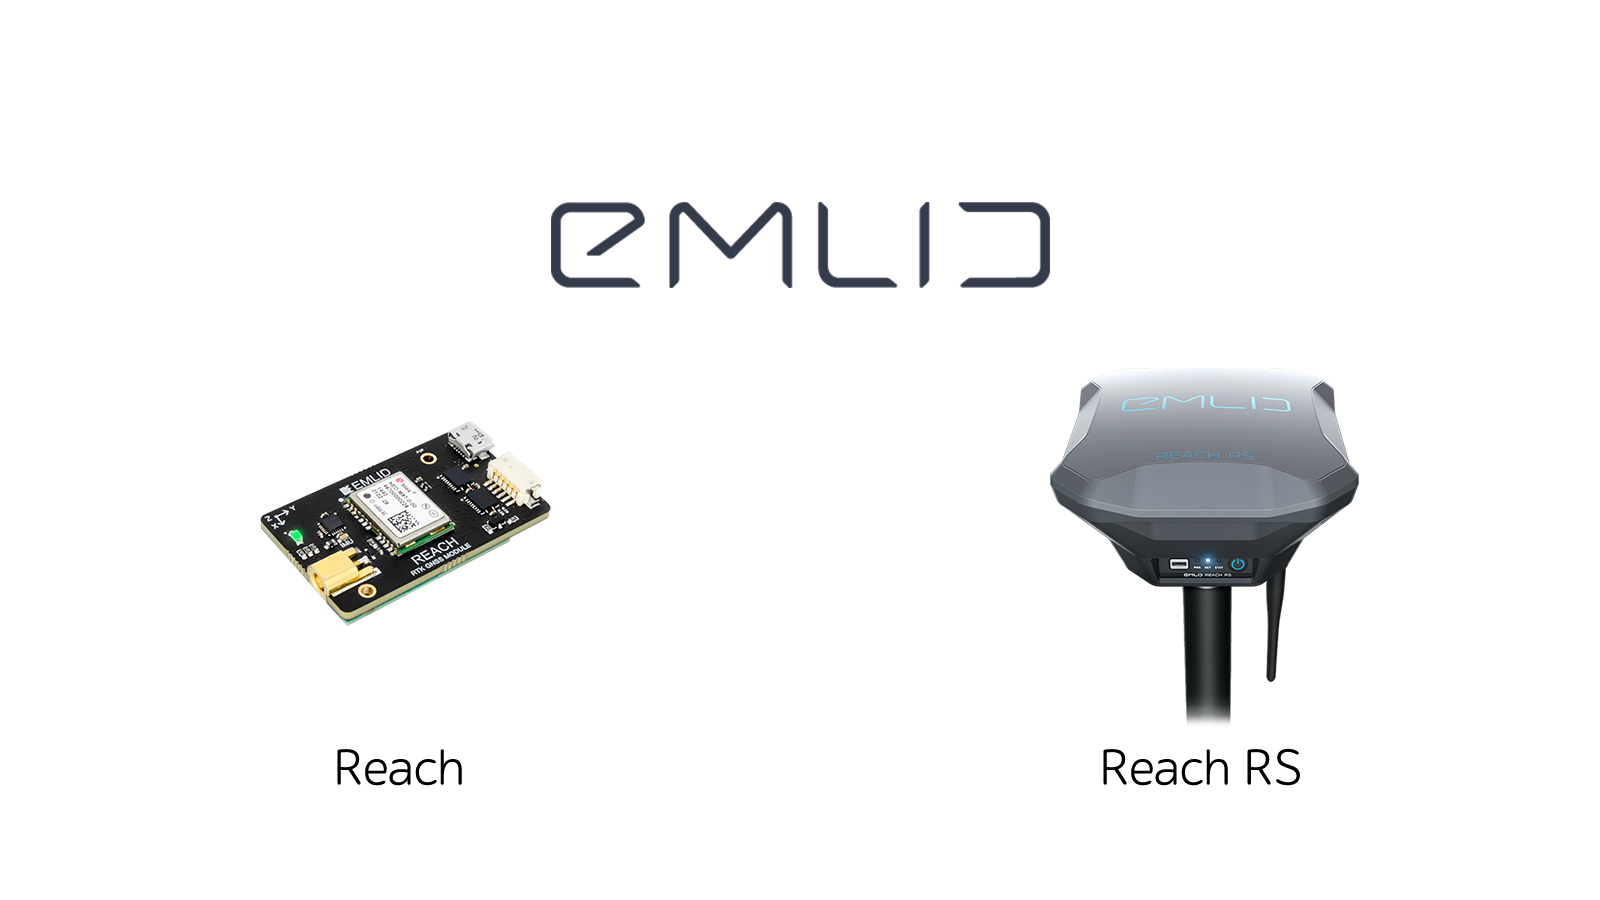
\includegraphics[width=\paperwidth]{../img/presentation/emlid-devices}
  }

  \begin{frame}
    \frametitle{Платформа для разработки}
  \end{frame}
}

%
% Required features
%
\begin{frame}
  \frametitle{Основные требования к веб-приложению}
  
  \large
  
  \begin{itemize}
    \setlength\itemsep{0.5em}
    \item Одностраничное приложение
    \item Автоматическая подстройка под тип устройства
    \item Адаптивность и кроссбраузерность
  \end{itemize}
  \begin{center}
    \vskip -0.7cm
    \color{ifmoblue}{\rule{.5\textwidth}{0.5pt}}
  \end{center}
  \vskip -0.5cm
  \begin{itemize}
    \setlength\itemsep{0.5em}
    \item \textbf{Возможность производить геодезические изыскания}
    \item Отображение информации в~соответствии с~текущей ролью в~RTK-системе
    \item Настройка режима RTK и~параметров приёмника
    \item Управление входными/выходными потоками данных
    \item Доступ к~логам данных и~их настройкам
    \item Настройка беспроводных соединений (Wi-Fi и~Bluetooth)
  \end{itemize}
\end{frame}


%
% System architecture
%
\begin{frame}
  \frametitle{Общая архитектура приложения}
  \vskip -0.5cm
  \begin{figure}[h]
    \centering
    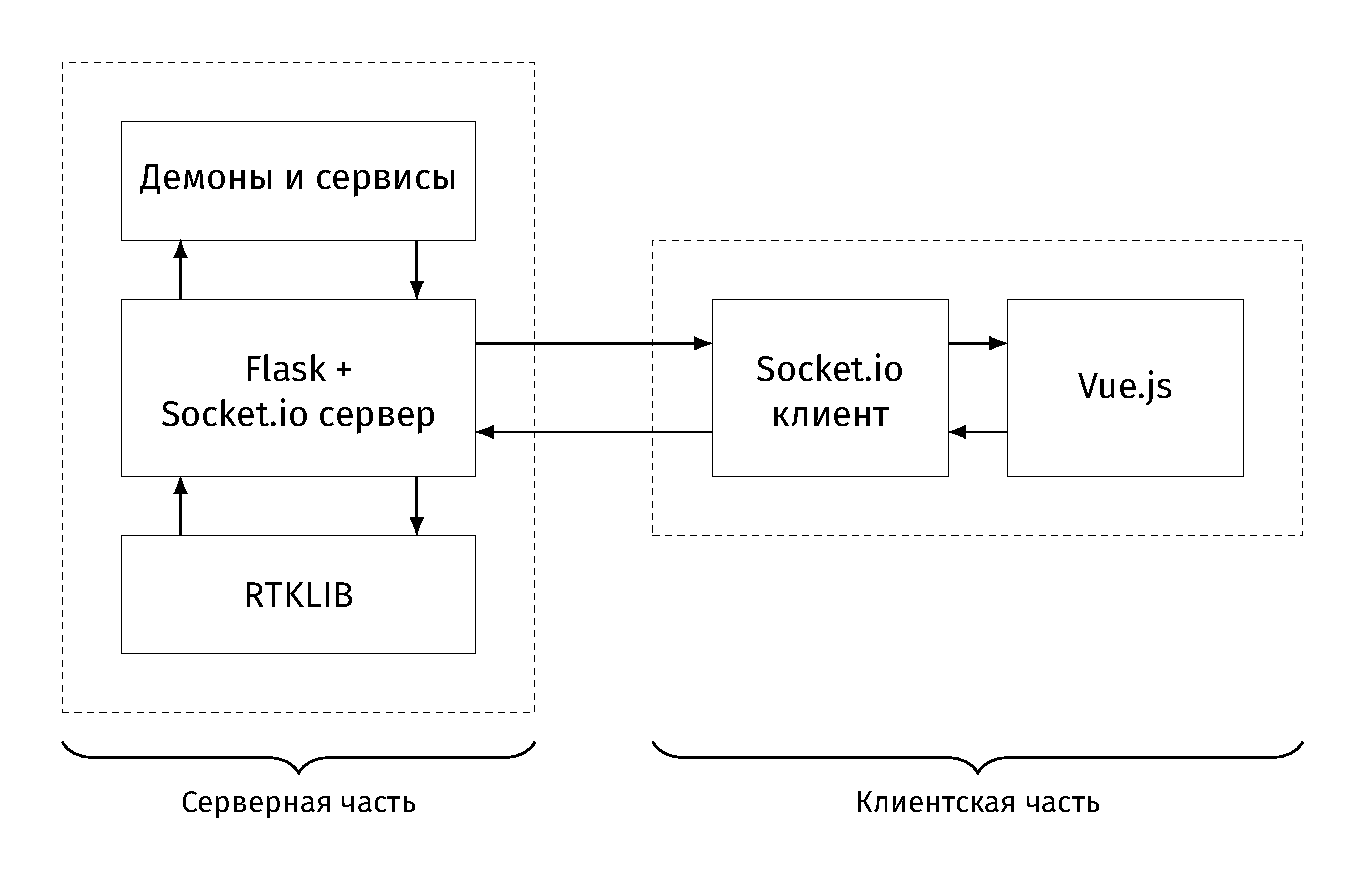
\includegraphics[width=.75\textwidth]{../img/tikz/system-architecture/pic_sans_no-border}
  \end{figure}
\end{frame}


%
% FE architecture
%
\begin{frame}
  \frametitle{Архитектура клиентской части приложения}
  \vskip -0.25cm
  \begin{figure}[h]
    \centering
    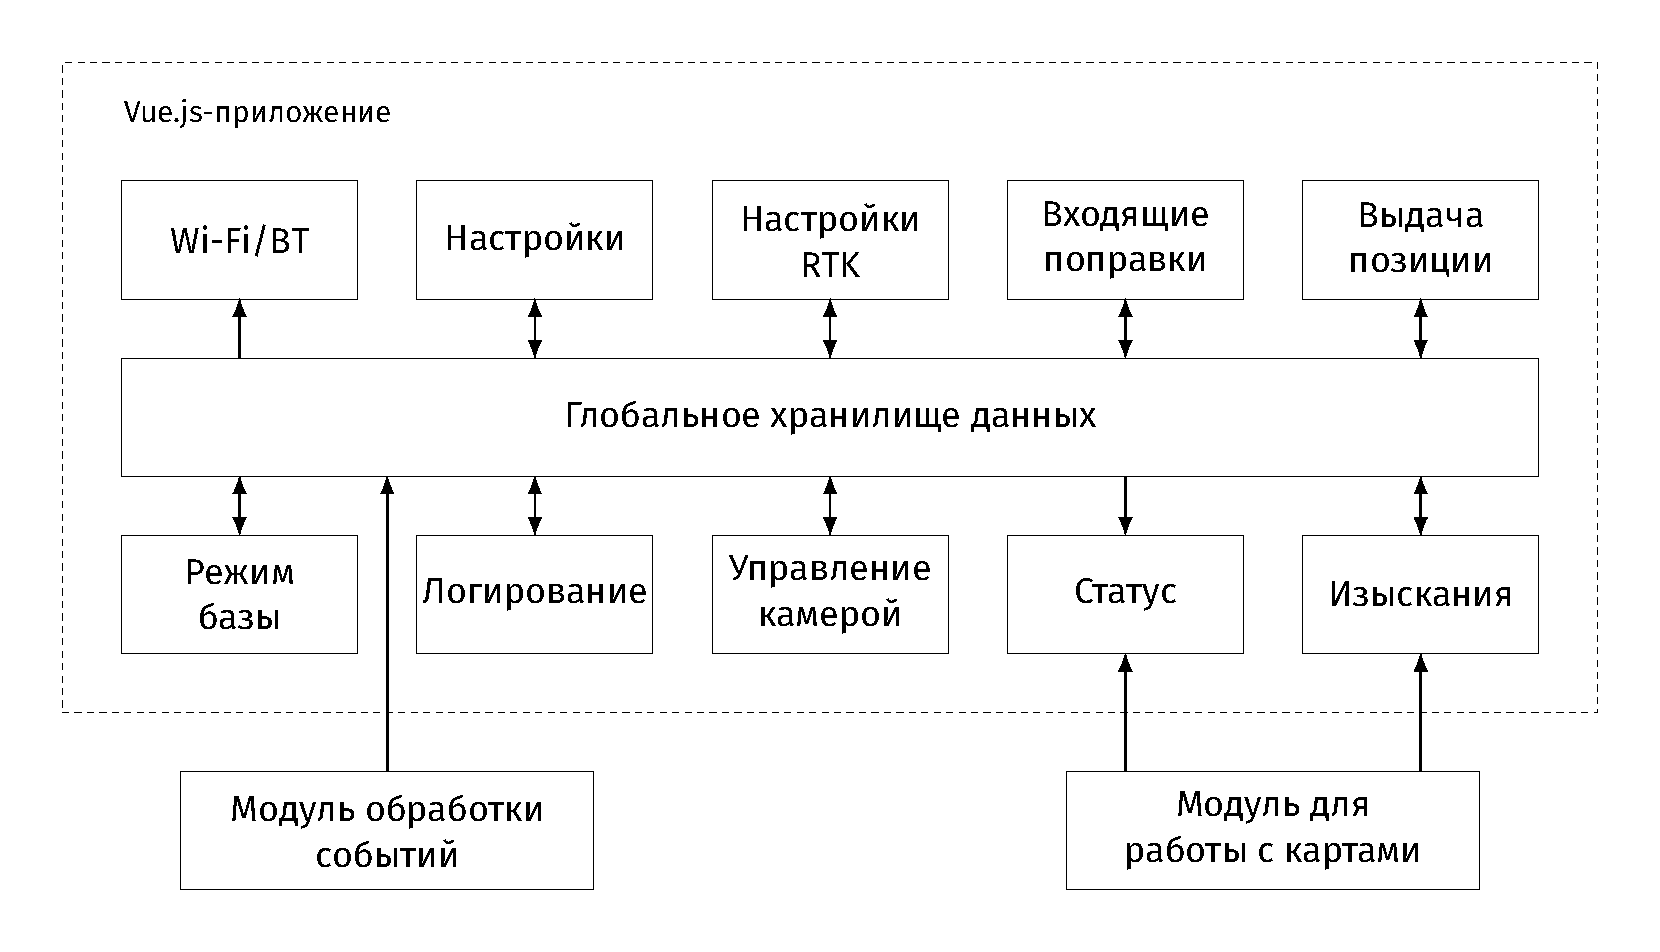
\includegraphics[width=.9\textwidth]{../img/tikz/fe-architecture/pic}
  \end{figure}
\end{frame}


%
% UI
%
\begin{frame}
  \frametitle{Разработка веб-приложения (\,1\,)}
  \framesubtitle{Адаптивный интерфейс}

  \begin{minipage}{\textwidth}
    \centering
    \begin{minipage}[c]{.5\textwidth}
      \centering
      \begin{figure}[c]
        \centering
        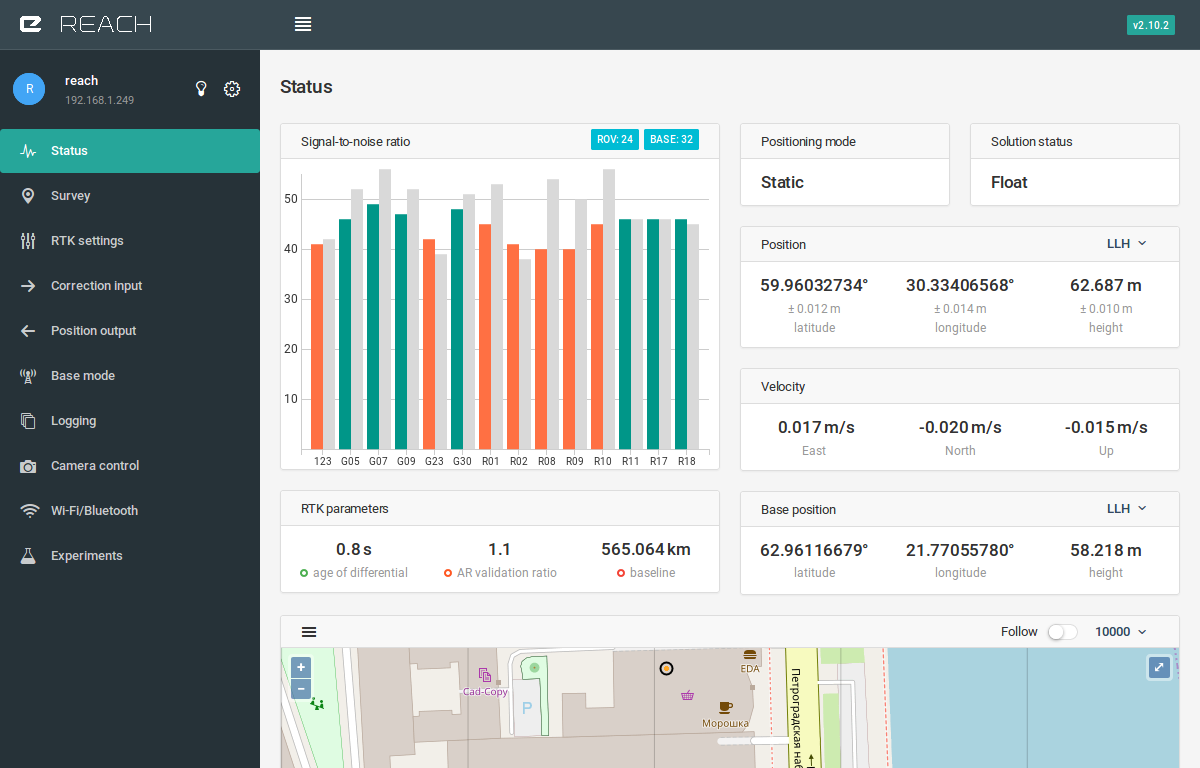
\includegraphics[height=4cm]{../img/reachview/homepage_responsive-lg}
      \end{figure}
    \end{minipage}
    \hspace{2em}
    \begin{minipage}[c]{.3\textwidth}
      \centering
      \begin{figure}[c]
        \centering
        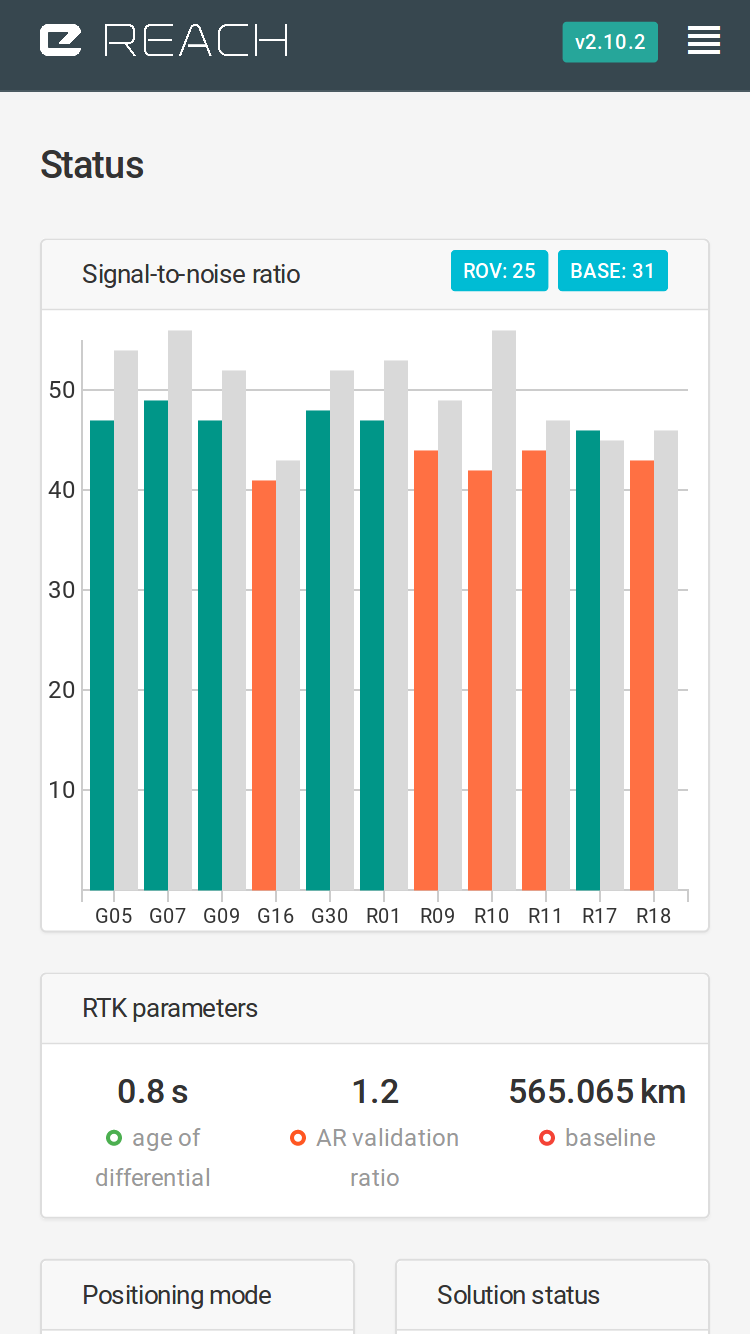
\includegraphics[height=5.5cm]{../img/reachview/homepage_responsive-xs}
      \end{figure}
    \end{minipage}
  \end{minipage}
\end{frame}


\setbeamercovered{transparent}

%
% Tabs
%
\begin{frame}
  \frametitle{Разработка веб-приложения (\,2\,)}
  \framesubtitle{Разделение интерфейса на секции}

  \begin{columns}[T]
%    \centering
%    \footnotesize
%    \vskip -1cm
    \begin{column}[T]{.32\textwidth}
      \begin{itemize}
        \item<1> Статус
        \item<2> Изыскания
        \item<3> Настройки RTK
        \item<4> Входящие поправки
        \item<5> Выдача позиции
        \item<6> Режим базы
        \item<7> Логирование
        \item<8> Управление камерой
        \item<9> Wi-Fi/Bluetooth
        \item<10> Настройки
      \end{itemize}
    \end{column}
    \hspace{1em}
    \begin{column}{.64\textwidth}
      \only<1>{
        \begin{figure}[c]
          \centering
          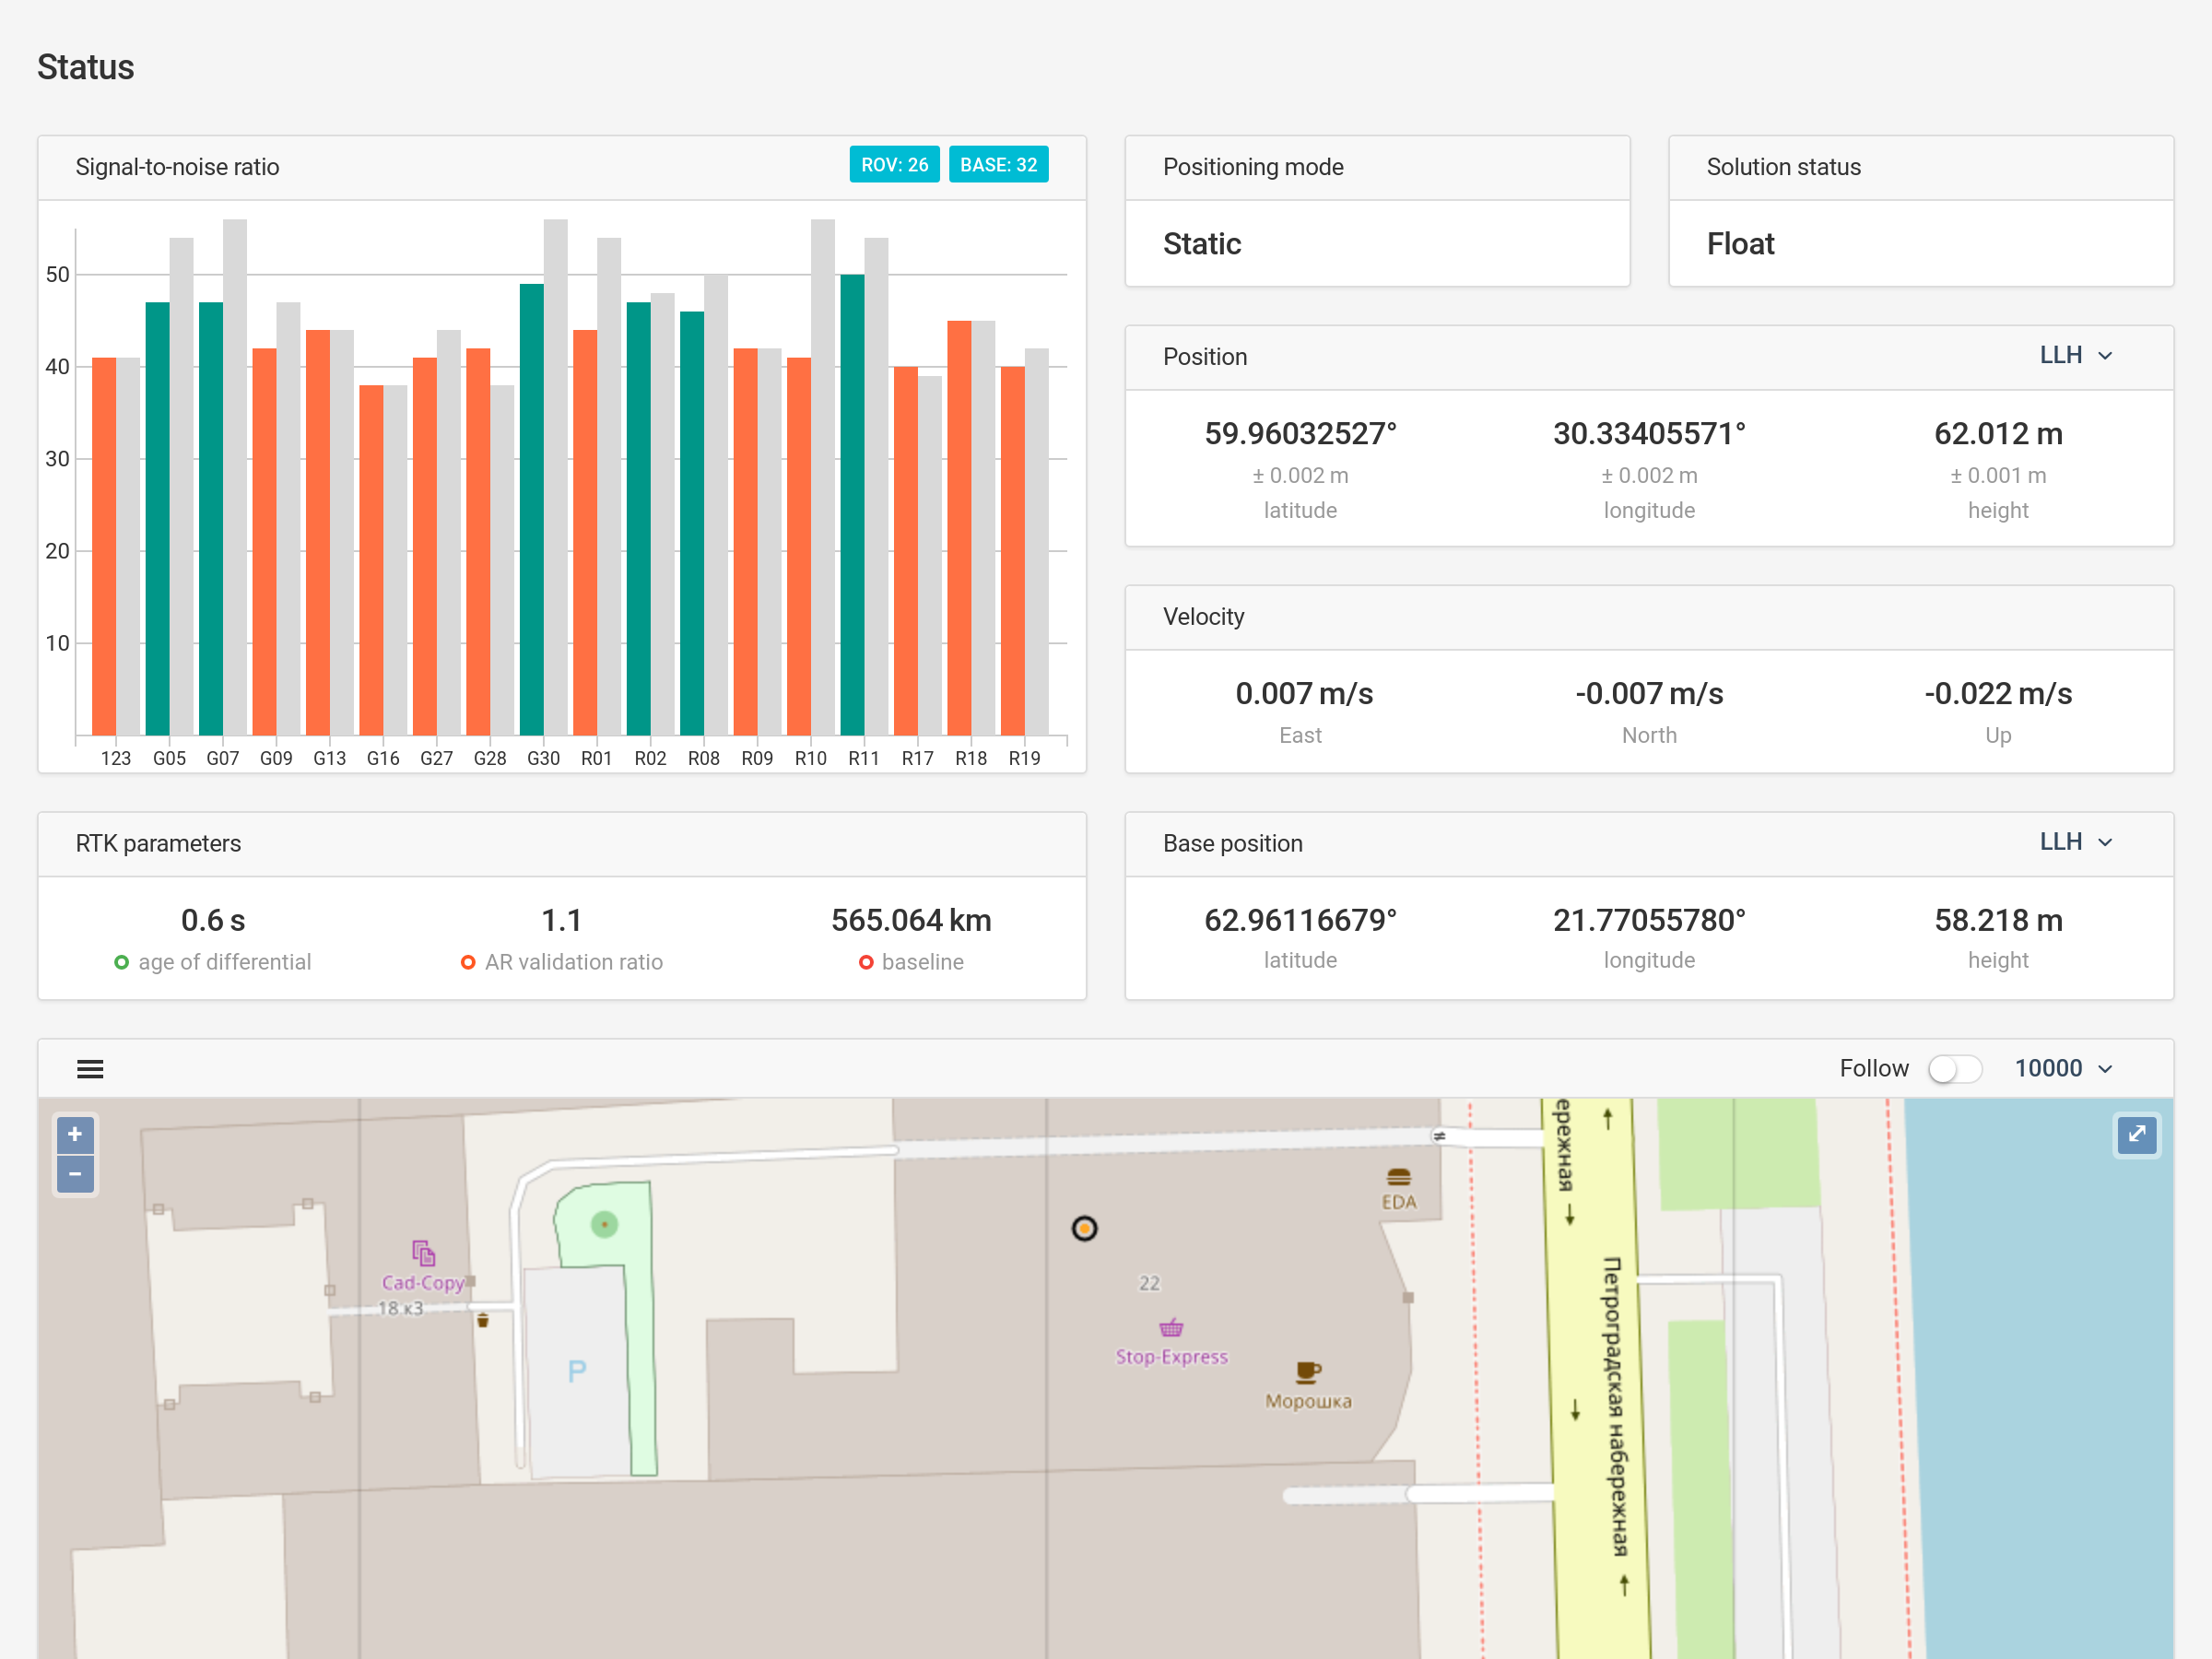
\includegraphics[height=5.5cm]{../img/reachview/status_content_laptop}
        \end{figure}
      }
      \only<2>{
        \begin{figure}[c]
          \centering
          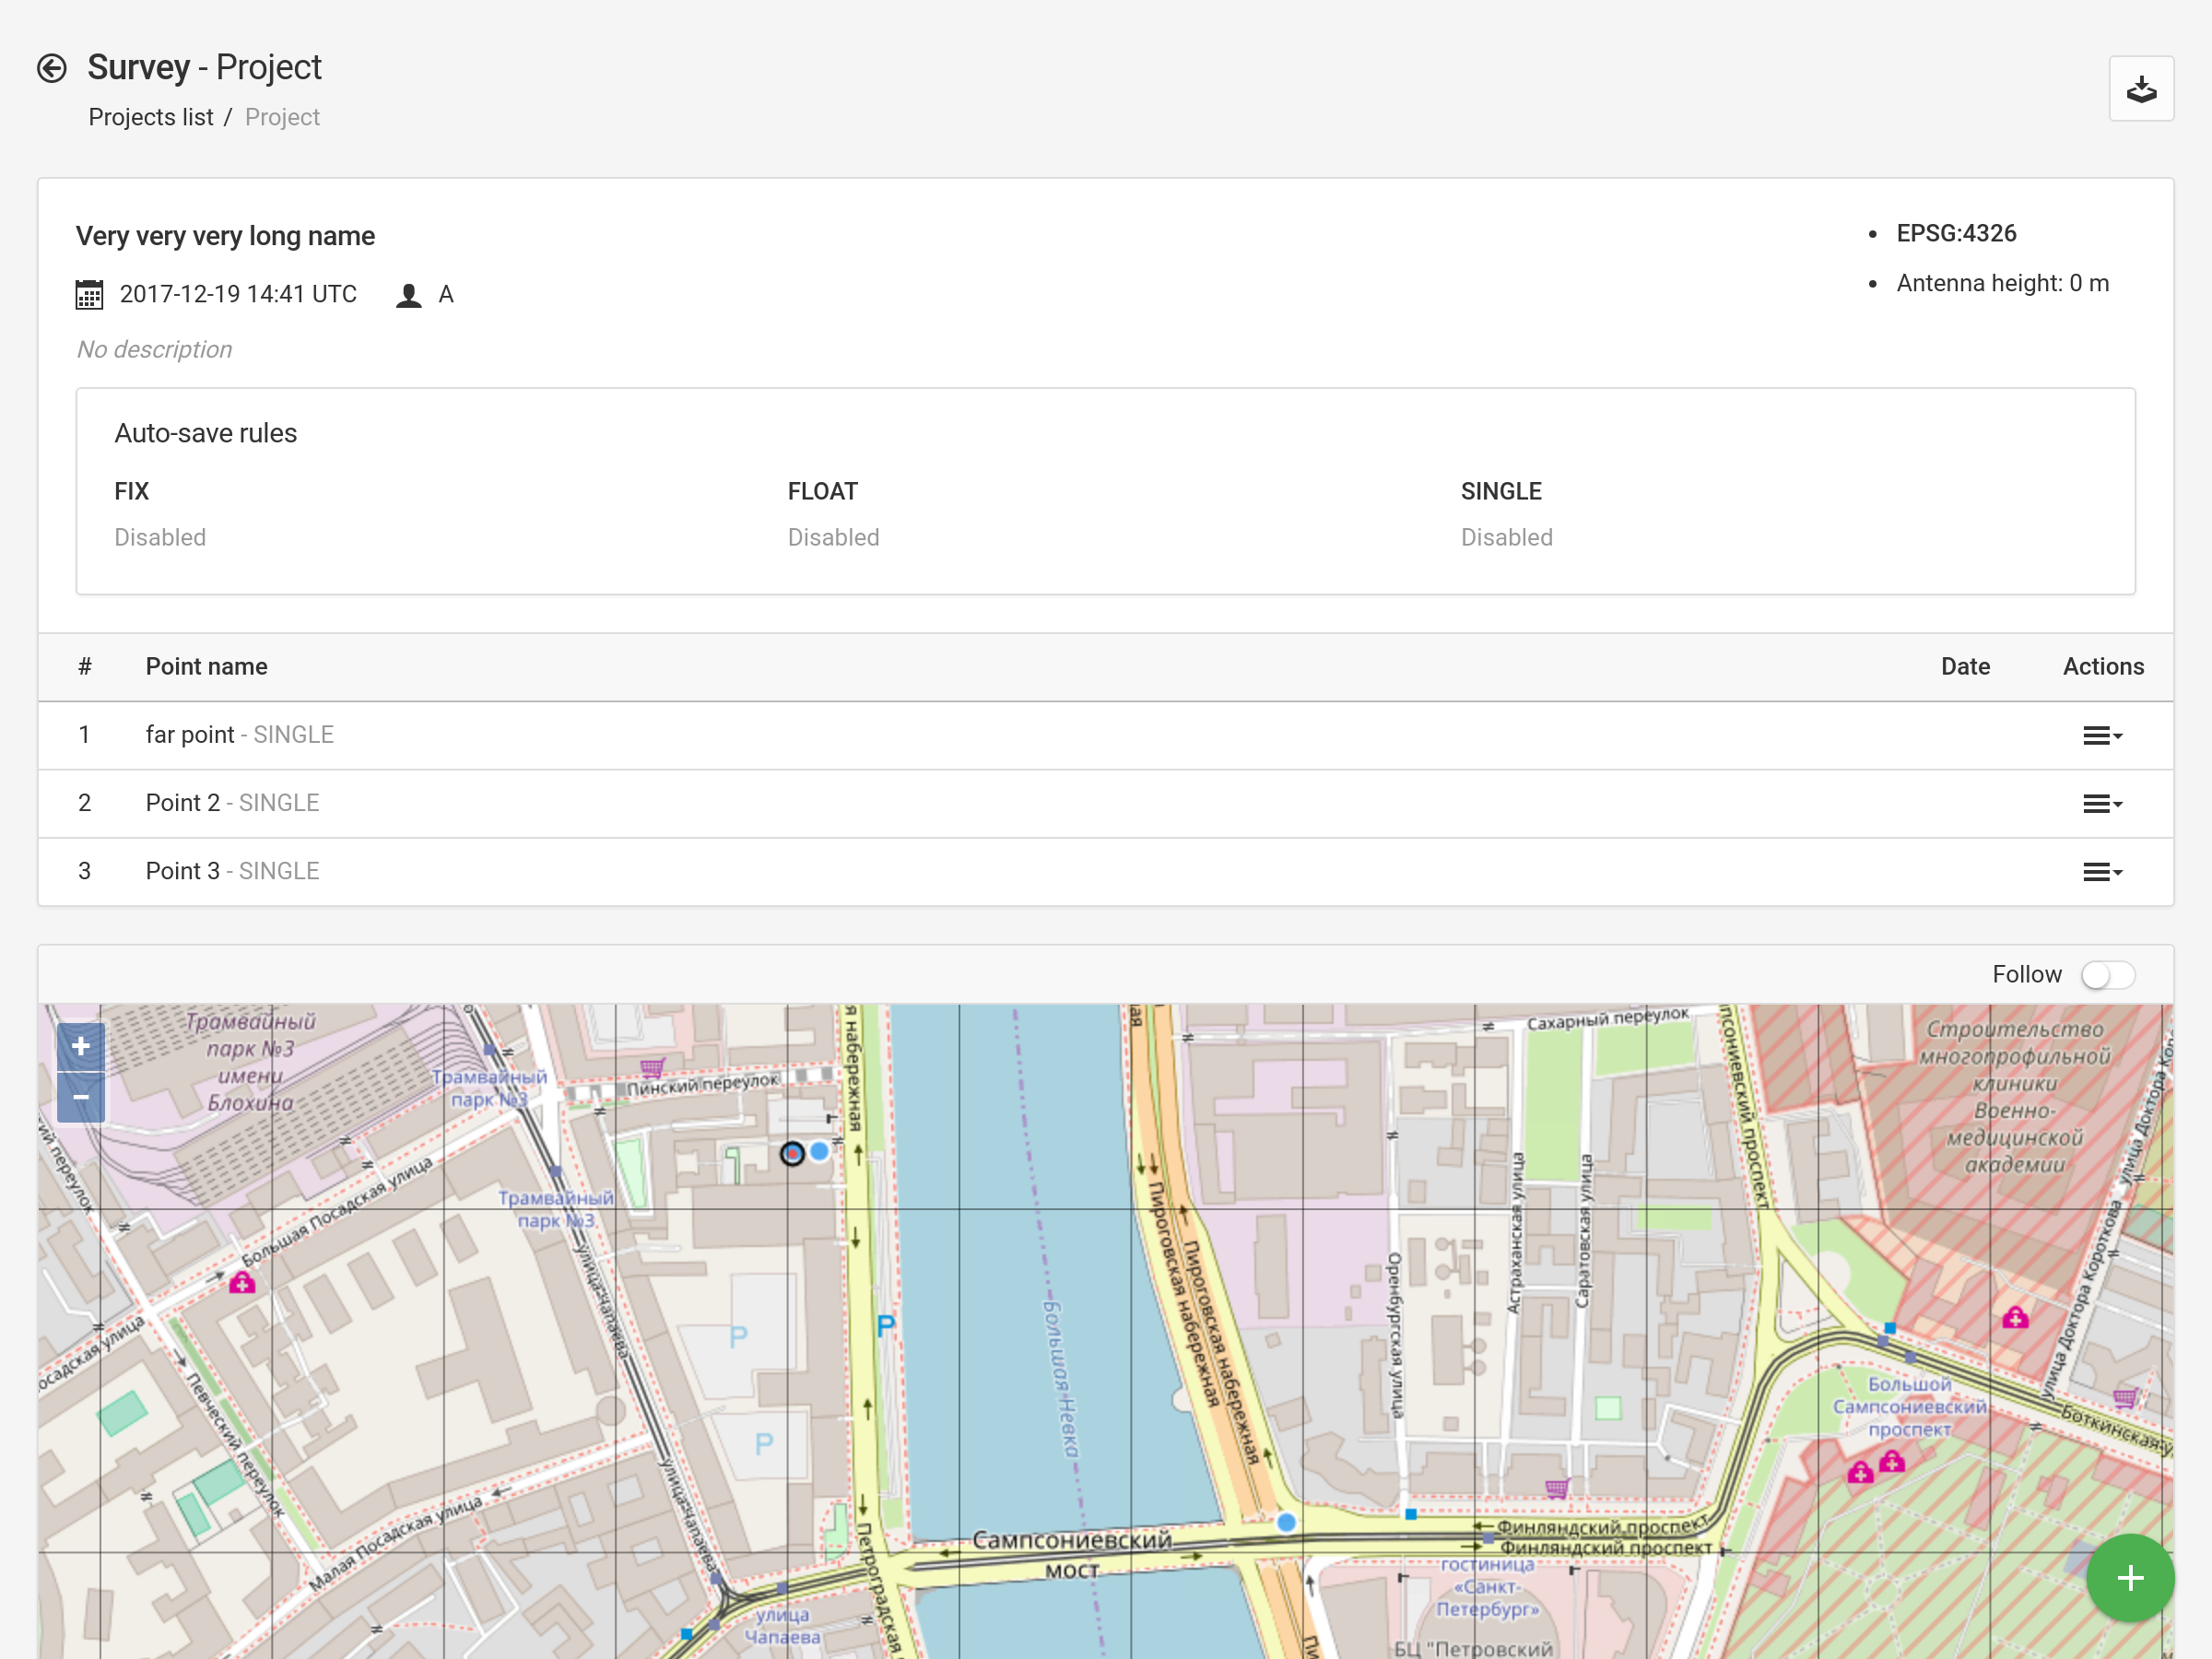
\includegraphics[height=5.5cm]{../img/reachview/survey_content_laptop}
        \end{figure}
      }
      \only<3>{
        \begin{figure}[c]
          \centering
          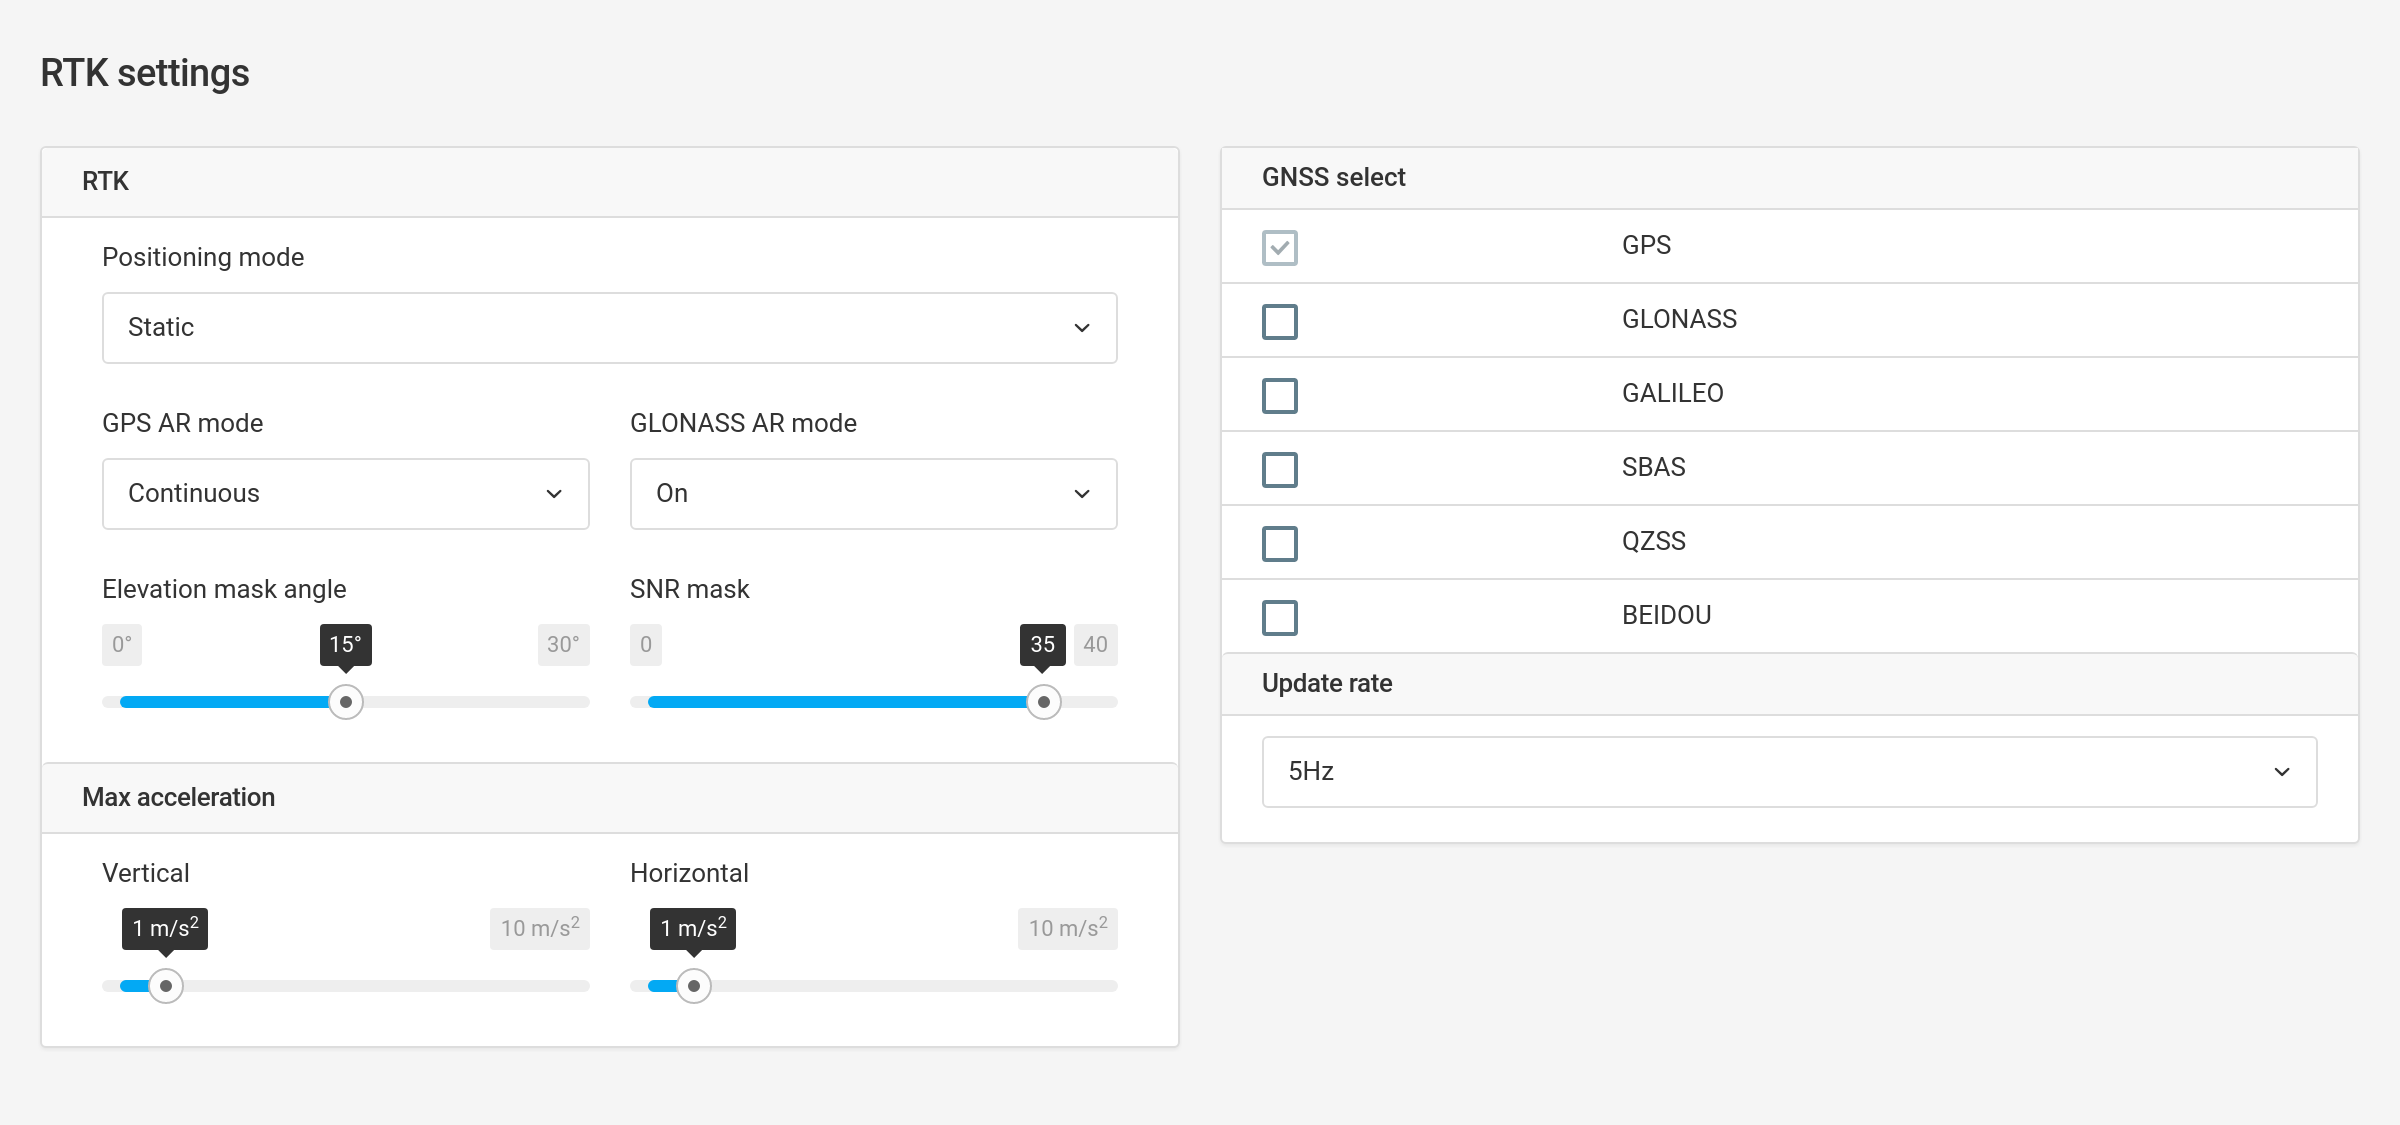
\includegraphics[height=4.25cm]{../img/reachview/rtk-settings_content_laptop}
        \end{figure}
      }
      \only<4>{
        \begin{figure}[c]
          \centering
          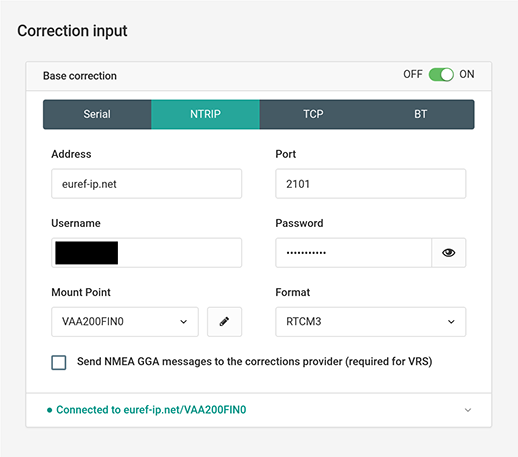
\includegraphics[height=5.5cm]{../img/reachview/correction-input_content_laptop}
        \end{figure}
      }
      \only<5>{
        \vskip 1cm
        \begin{figure}[c]
          \centering
          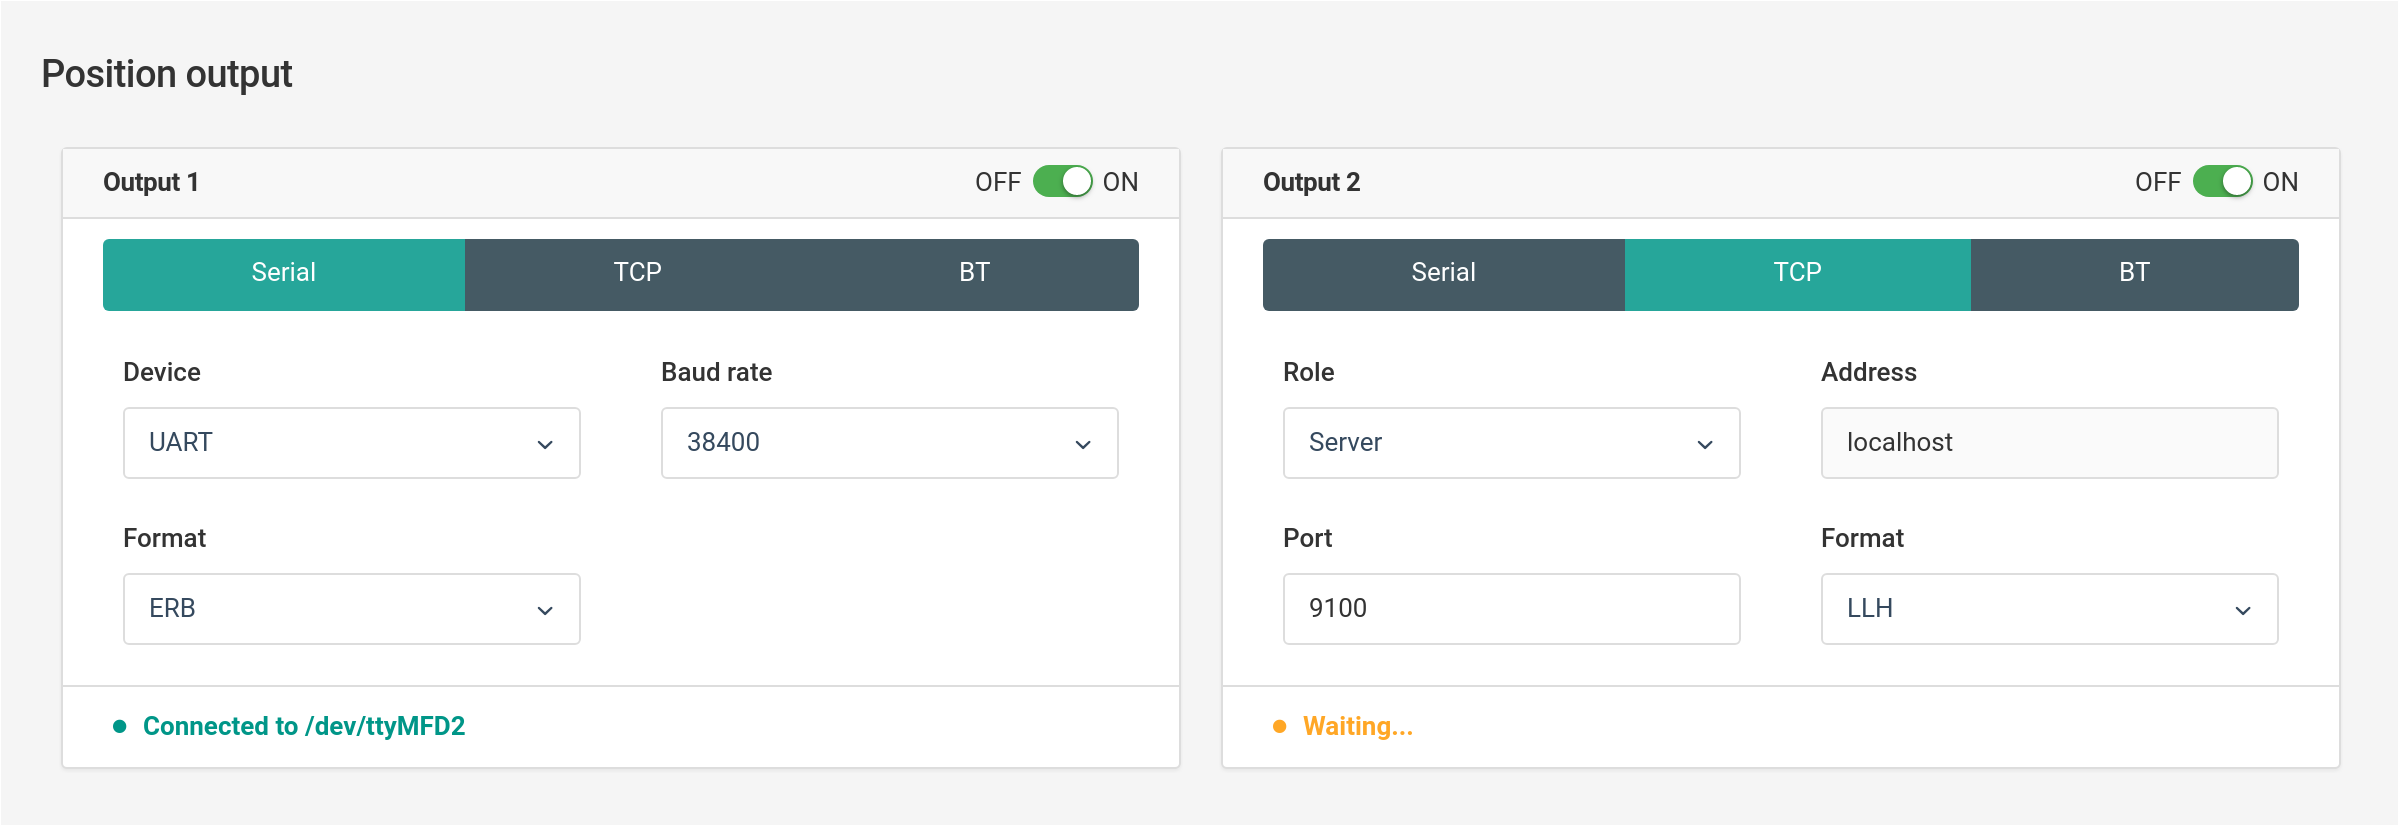
\includegraphics[height=3cm]{../img/reachview/position-output_content_laptop}
        \end{figure}
      }
      \only<6>{
        \begin{figure}[c]
          \centering
          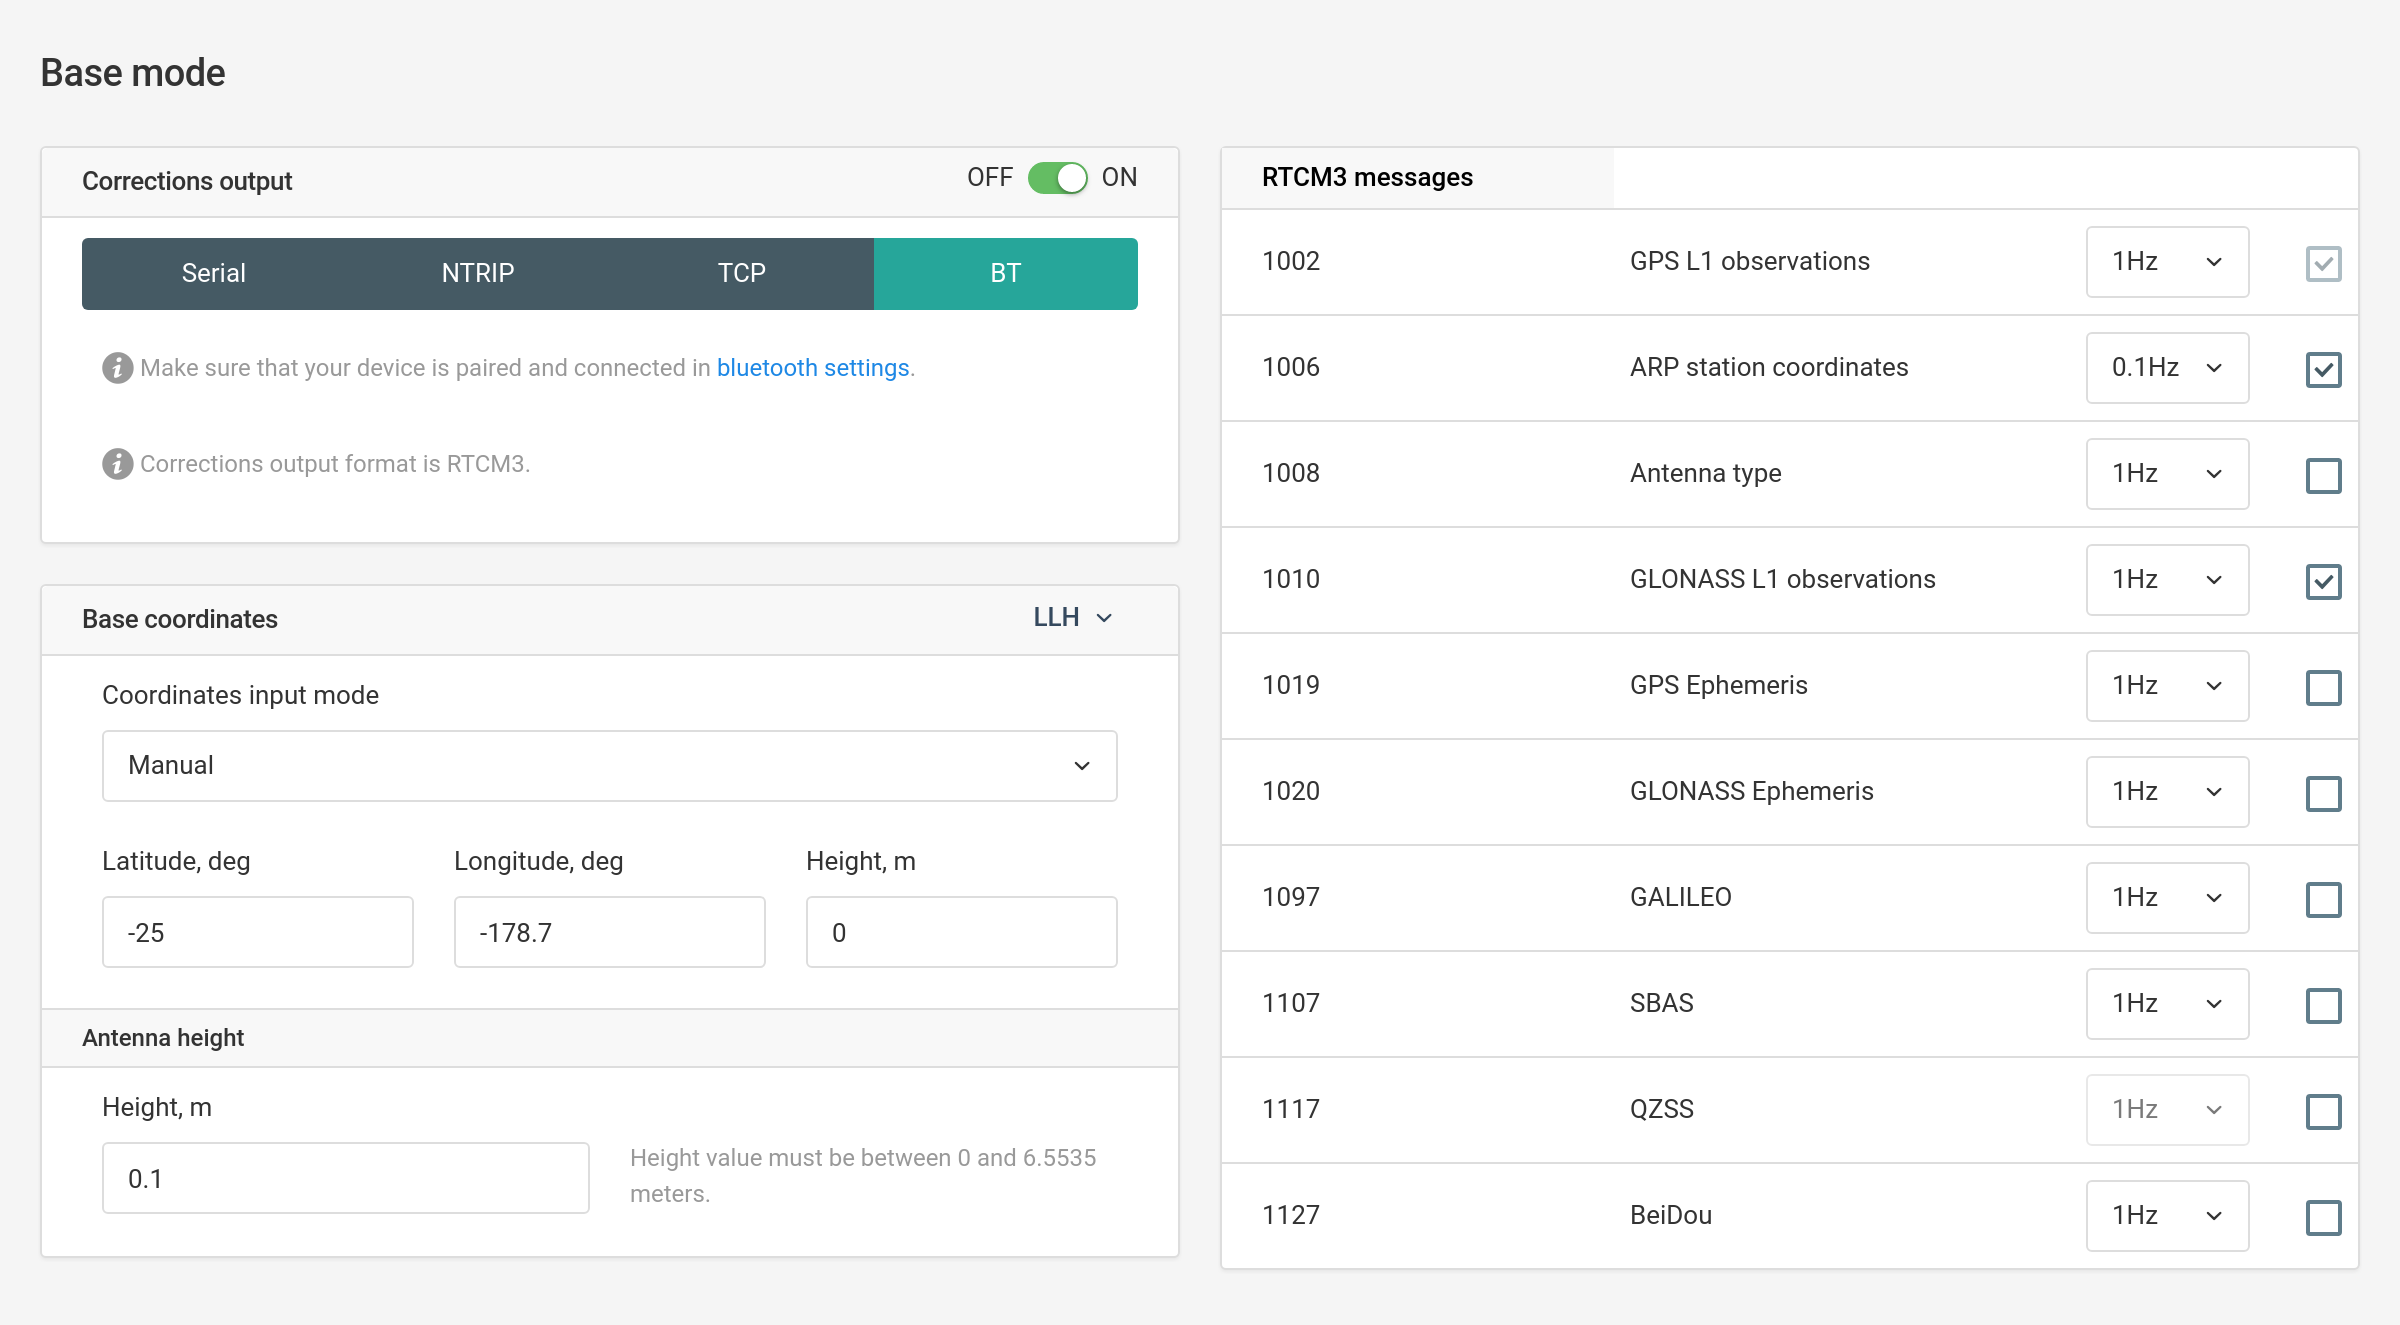
\includegraphics[height=5cm]{../img/reachview/base-mode_content_laptop}
        \end{figure}
      }
      \only<7>{
        \begin{figure}[c]
          \centering
          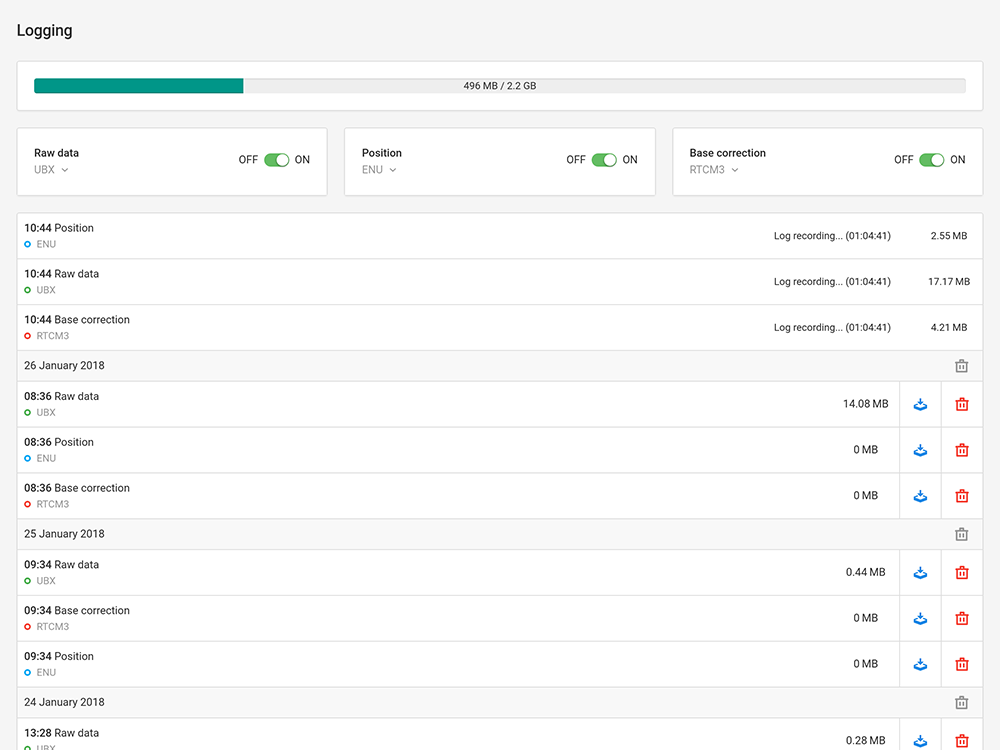
\includegraphics[height=5.5cm]{../img/reachview/logging_content_laptop}
        \end{figure}
      }
      \only<8>{
        \vskip 0.5cm
        \begin{figure}[c]
          \centering
          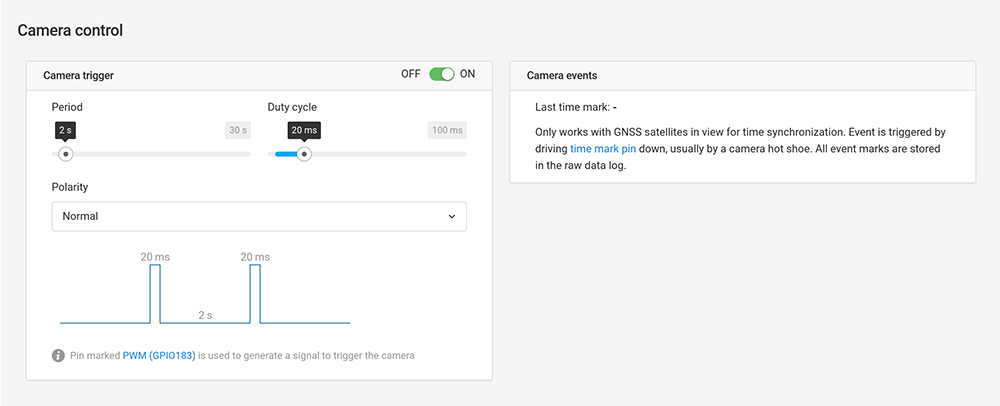
\includegraphics[height=3.5cm]{../img/reachview/camera-control_content_laptop}
        \end{figure}
      }
      \only<9>{
        \begin{figure}[c]
          \centering
          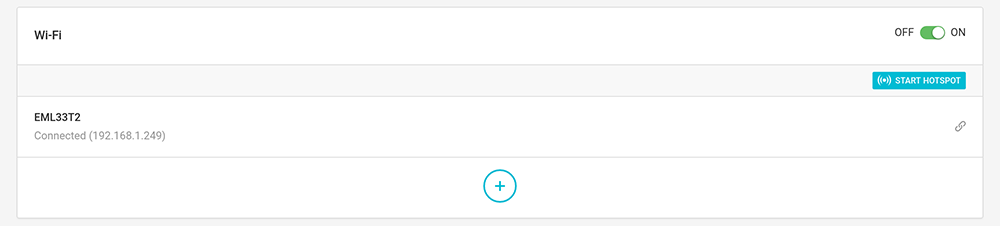
\includegraphics[width=.8\textwidth]{../img/reachview/wifi_content_laptop}\\
          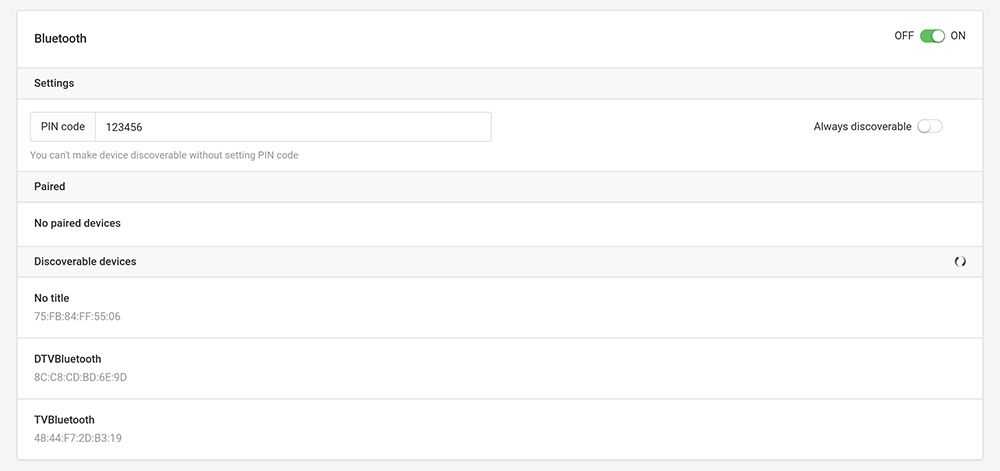
\includegraphics[width=.8\textwidth]{../img/reachview/bt_content_laptop}
        \end{figure}
      }
      \only<10>{
        \begin{figure}[c]
          \centering
          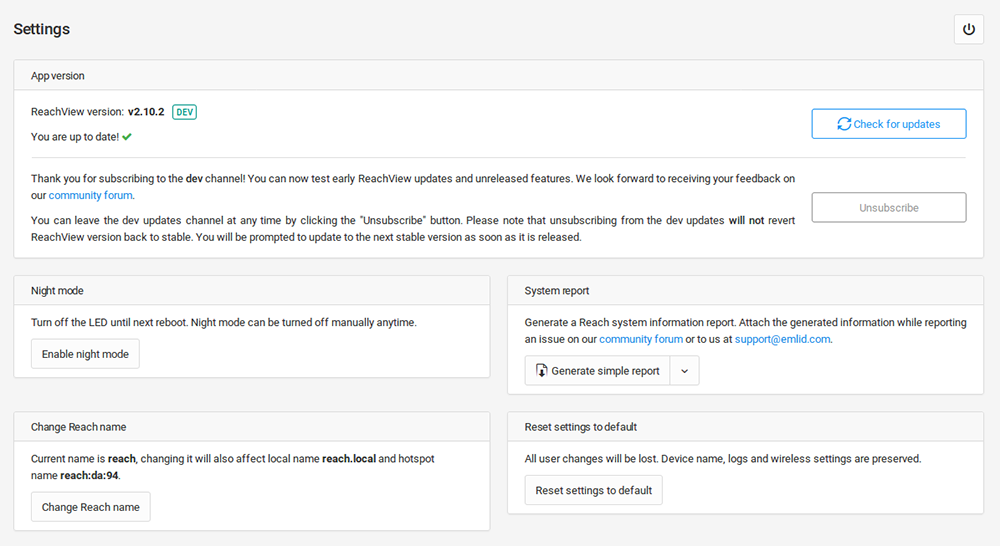
\includegraphics[height=4.75cm]{../img/reachview/settings_content_laptop}
        \end{figure}
      }
    \end{column}
  \end{columns}
\end{frame}


%
% Testing
%
\begin{frame}
  \frametitle{Тестирование и апробация приложения}
  
  \large
  
  \begin{itemize}
    \setlength\itemsep{0.5em}
    \item Модульные тесты
    \item Функциональные тесты
  \end{itemize}
  \begin{center}
    \vskip -0.5cm
    \color{ifmoblue}{\rule{.5\textwidth}{0.5pt}}
  \end{center}
  \vskip -0.2cm
  \begin{itemize}
    \setlength\itemsep{0.5em}
    \item[1.] Полевые испытания
    \item[2.] Beta-версии приложения для пользователей (с отзывами на форуме)\\
              Получение отзывов инициативной группы опытных геодезистов
    \item[3.] Разработанное приложение принято основной рабочей версией веб-интерфейса для Reach и~Reach~RS
  \end{itemize}
  \vskip -0.2cm
  \begin{figure}[b]
    \centering
    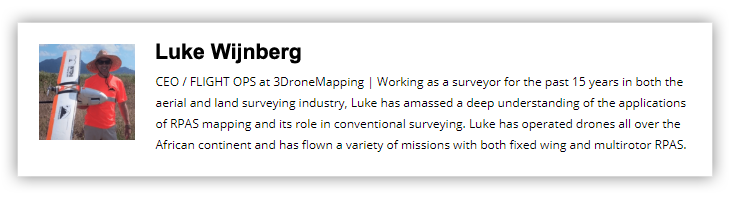
\includegraphics[width=.5\paperwidth]{../img/presentation/luke_wijnberg}
  \end{figure}
\end{frame}


%
% Results
%
\begin{frame}
  \frametitle{Результаты}

  \large

  \begin{itemize}
    \setlength\itemsep{0.5em}
    \item[1.] Проведён обзор областей применения высокоточного позиционирования;
    \item[2.] Рассмотрены проблемы доступности профессионального геодезического оборудования и слабой распространённости пакета RTKLIB;
    \item[3.] Проведён анализ применения веб-интерфейсов для взаимодействия с~устройствами без органов управления;
    \item[4.] Создано веб-приложение для взаимодействия пользователя с~программным пакетом RTKLIB, встроенным в~устройства Emlid Reach и~Emlid Reach~RS;
    \item[5.] Созданное приложение протестировано и~успешно внедрено;
    \item[6.] Налажен процесс общения с~пользователями, что позволяет получать отзывы, пожелания и~отчёты об ошибках;
    \item[7.] Создано два канала получения обновлений приложения.
  \end{itemize}
\end{frame}


%
% The End
%
{
  \setbeamertemplate{footline}{}

  \begin{frame}[c]
    \begin{center}
      \Huge\bfseries
      \color{ifmoblue}{Спасибо за внимание}
    \end{center}
  \end{frame}
}

\end{document}
